\documentclass[a4paper,11pt]{article}
\usepackage[T1]{fontenc}
\usepackage[utf8]{inputenc}
\usepackage{lmodern}
\usepackage[toc,page]{appendix}
\input GetPackages

\title{MICE Target Simulation}
\author{Tom Lord, Paolo Franchini}

\begin{document}

\maketitle
\tableofcontents

\begin{abstract}
Simulation of the pion production coming out from the MICE target using the MARS simulation software and implementation of this simulation into the MICE Monte Carlo software.
\end{abstract}

\newpage

\section{Motivation}

Non trivial discrepancies in the data versus Monte Carlo comparison have justified the necessity to reconsider the pions momentum distribution used as primary input of the MICE Monte Carlo.
The former model consisted in a fit done with three Gaussian of a pion distribution produced in 2008 with a earlier version of the MARS simulation software. Lack of documentation on this first study made it hard to evaluate the goodness of the model that shows a peculiar hard cut in the distribution.

The MICE target has been described in its major components using the MARS simulation software.
\section{The MICE target in the ISIS proton beam}

%Brief description of the MICE target.\\
The MICE target operates parasitically on protons undergoing acceleration within the ISIS synchrotron, dipping into the low-density halo of the beam on selected pulses just prior to their extraction, with an ~1 Hz frequency. It is designed as a bored TiAl cylinder with inner radius 2.275 cm and outer radius 2.975 cm. The resulting thickness of material for proton collisions is significantly lower than one interaction length (~27.8cm for titanium), giving an interaction probability of order ~1\%. As a result, order 1E12 simulated ISIS protons are required for sufficient statistics. 

%ISIS proton beam: energy, dimension, position...\\
The ISIS synchrotron circulates two beam bunches of approximately 1.4E13 protons each per cycle, with these undergoing close to 10,000 revolutions before extraction in a circulation time of 10ms. Proton beam-size shrinking between radii of ~67mm and 48mm during it's acceleration through the synchrotron results in proton collision energy and beamwidth both varying in time with respect to the initial ISIS proton injection trigger, as well as due to small field fluctuations. Hence the target undergoes many proton collisions of between 650MeV and 800MeV collision energy during each dip (See Table \ref{Table:Inj}). 

\begin{table*}
\centering
\label{Table:Inj}
\begin{tabular}{ c c }
\hline Time after injection (ms) & Proton Energy (MeV) \\
\hline \vspace{-2.5mm} \\
$7.0$ & $615.59$ \\ \hline
$7.1$ & $626.53$ \\
$7.2$ & $637.25$ \\
$7.3$ & $647.73$ \\
$7.4$ & $657.96$ \\
$7.5$ & $667.93$ \\
$7.6$ & $688.62$ \\
$7.9$ & $687.02$ \\
$7.8$ & $696.12$ \\
$7.9$ & $704.90$ \\ \hline
$8.0$ & $713.35$ \\ \hline
$8.1$ & $721.47$ \\
$8.2$ & $729.23$ \\
$8.3$ & $736.64$ \\
$8.4$ & $743.68$ \\
$8.5$ & $750.33$ \\
$8.6$ & $756.60$ \\
$8.7$ & $762.48$ \\
$8.8$ & $767.95$ \\
$8.9$ & $773.01$ \\ \hline
$9.0$ & $777.65$ \\ \hline
$9.1$ & $781.87$ \\
$9.2$ & $785.66$ \\
$9.3$ & $789.02$ \\
$9.4$ & $791.94$ \\
$9.5$ & $794.41$ \\
$9.6$ & $796.44$ \\
$9.7$ & $798.02$ \\
$9.8$ & $799.15$ \\
$9.9$ & $799.83$ \\ \hline
$10.0$ & $800.06$ \\
\hline
\end{tabular}
\caption{Time after injection (ms) vs Proton Energy in the ISIS beam (MeV). Interactions from target dipping occur over this time range.}
\end{table*}

 Furthermore due to the field changes in the synchrotron, the ISIS beam often drifts from the well-defined beam center, such that the beam centre displacement (BCD) figure recorded is only a nominal value. 

As noted in \cite{micenote480} the target is operated through the RATS control software, allowing the user to alter both BCD and User Delay (defined from the machine start trigger + $(2^{n}\times20ms)-15ms$, with n some integer) s.t. dips travelling further to achieve lower BCD may operate with reduced User Delay to compensate. 

\section{MARS simulation}

The design of the MICE target, in particular the surrounding structure, is defined as in Fig. \ref{fig:MARSwindow}. The presented design has been based on schematics \cite{beampipesurvey1}\cite{beampipesurvey2}\cite{beampipesurvey3} and surveys \cite{ISISbeamlinesurvey}\cite{MICEsurvey}. The MICE beamline is orientated at 25 deg with respect to the ISIS beamline section where the target is located. In addition to the cylindrical bored-target structure from the previous model, various features of the surrounding ISIS beampipe structure have been included, such as the surrounding beampipe and target window structure oriented at 25 degrees toward the MICE beamline, as shown in Figs \ref{fig:MARSwindow}, \ref{fig:MARSXY}. An initial section of the MICE beampipe up to the Q1 aperture (approx 2.5m downstream) is also modelled in MARS as in \ref{fig:MARSXZ}. For efficient runtime, particles are selected at 1m from the target IP inside the MICE beampipe. This produces the resulting pion distribution which is fitted and passed to G4BL. Comparison was made with some output taken 2m downstream, however this showed little change to the observed momentum distribution.

As both BCD and User Delay are altered live by the MICE operator to respond to ISIS beam drift \& target deterioration in order to optimise statistics, modelling of an exact dip cycle to replicate target dip throughout the entire MICE data collection is difficult. Instead a number of model iterations with varying proton energy and beamwidth have been simulated to compare pion production, momentum distribution \& results from downstream propagation. This is shown in Fig. \ref{fig:PiMomentum}. 

\begin{figure}[t!]
  \begin{center}
    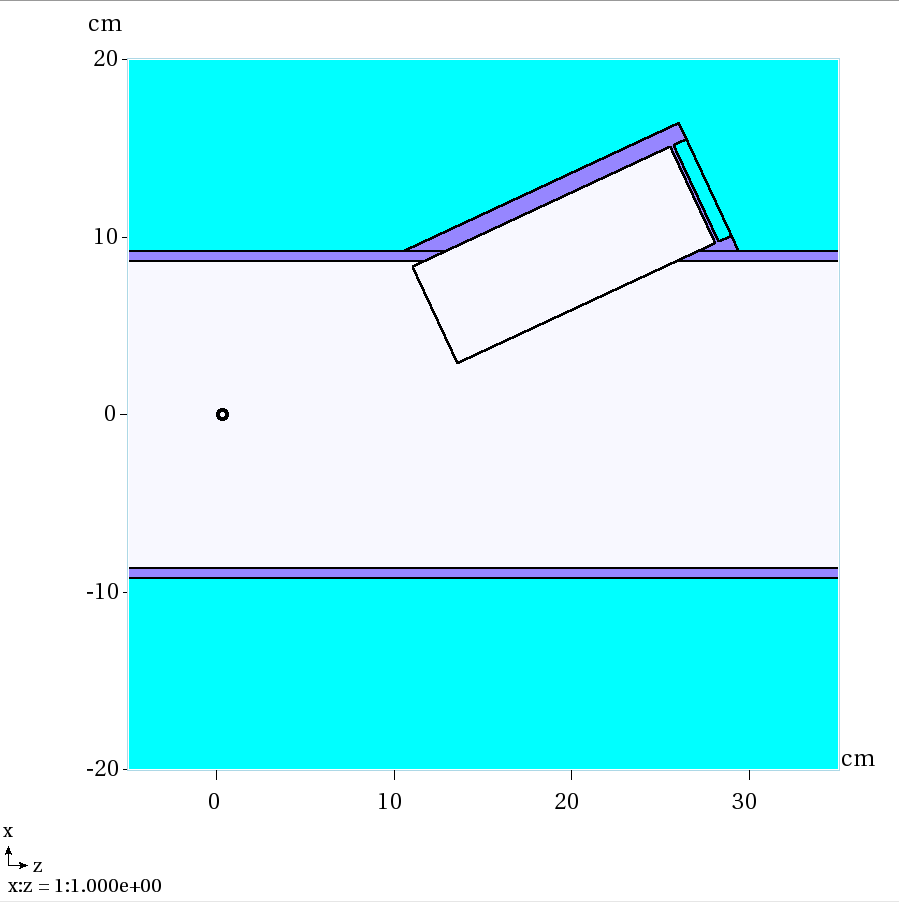
\includegraphics[width=1.0\columnwidth]{./figures/XZGeom-v6-Q1-y=6cm-Zoom.png}
    \caption{Design of the target in the MARS simulation. ( require z=60cm?along the x-axis? ) }
    \label{fig:MARSwindow}
  \end{center}
\end{figure}

\begin{figure}[t!]
  \begin{center}
    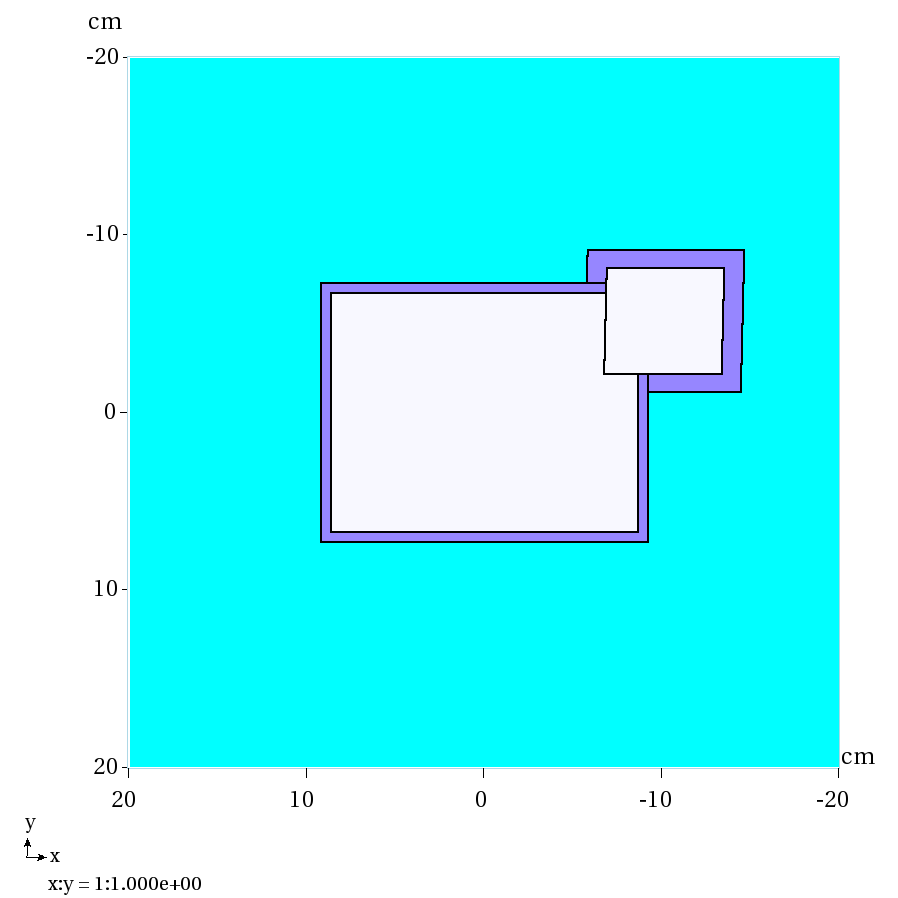
\includegraphics[width=1.0\columnwidth]{./figures/XYGeom-v6-Q1-z=22cm.png}
    \caption{Design of the target in the MARS simulation. STST304 structures are shown in purple, with the pink ring at (0,0) the cross-sectional slice of the TiAl target taken at some y>0. ( require z=60cm?along the x-axis? ) }
    \label{fig:MARSXY}
  \end{center}
\end{figure}

\begin{figure}[t!]
  \begin{center}
    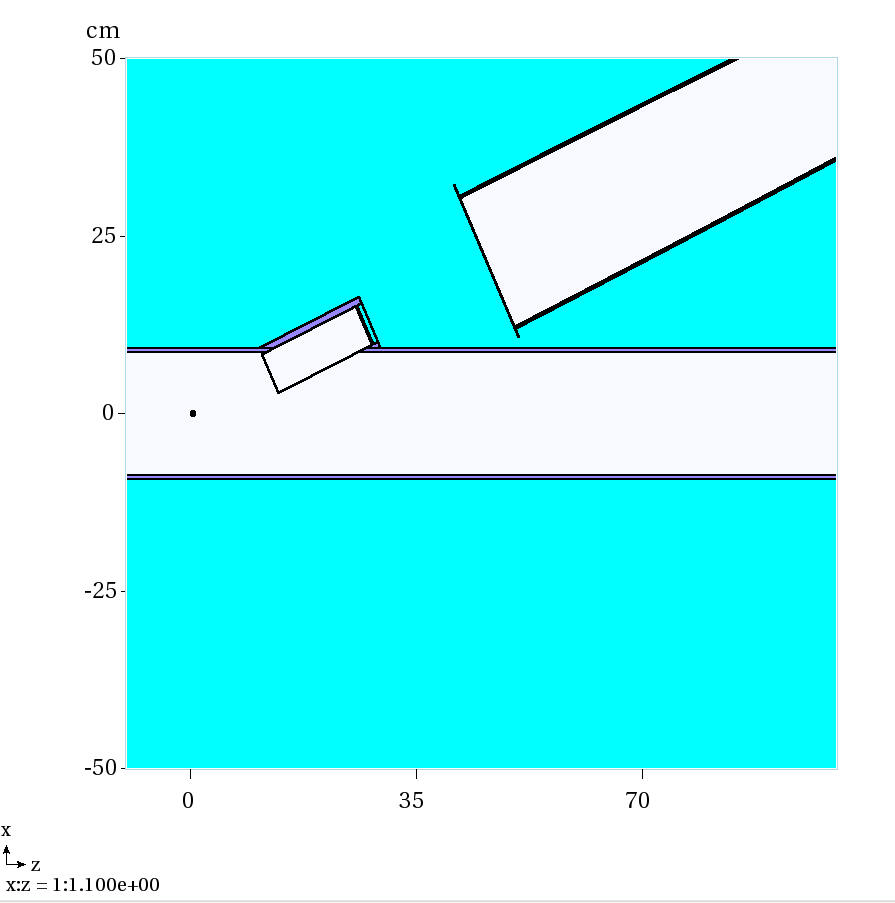
\includegraphics[width=1.0\columnwidth]{./figures/XZGeom-v6-Q1-y=6cm.png}
    \caption{MICE target inside ISIS beampipe, alongside MICE beampipe in the MARS simulation. }
    \label{fig:MARSXZ}
  \end{center}
\end{figure}

\begin{figure}[t!]
  \begin{center}
    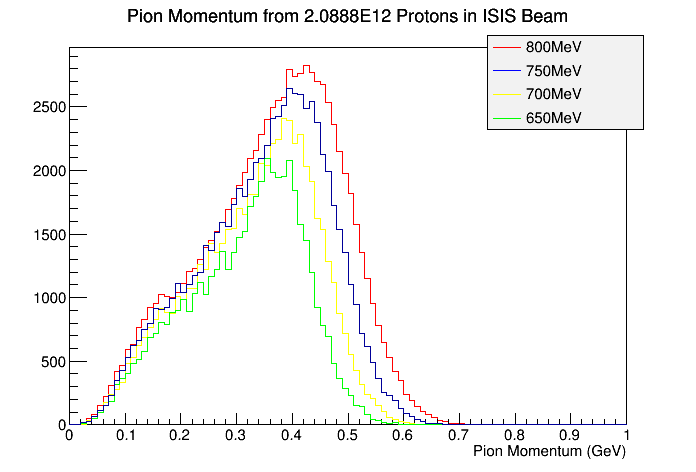
\includegraphics[width=1.0\columnwidth]{./figures/PiMomentumNew.png}
    \caption{Momentum of $\pi^{+}$ produced in Proton-target collisions, taken 1m downstream in the MICE beamline.}
    \label{fig:PiMomentum}
  \end{center}
\end{figure}


\section{MAUS simulation}

The Monte Carlo in MICE is produced in a two-step process. In the first step a pion beam is produced according to an initial momentum distribution and is propagated using G4BL up to the bending dipole D2. After this point MAUS takes over propagating the particles (pions, muons and electrons coming from decays) through the remaining part of the beamline up to the EMR, passing through the cooling channel, according to the geometry and run selected to be simulated. 

\subsection{Monte Carlo and data comparison}

A few figures of merit have been considered: time of flight of the particles between TOF0 and TOF1 and momentum distribution of pions and muons in the upstream tracker at station 5.
Simulations have been produced for 140, 200 and 240 MeV/c nominal pionic beams, with further planned.  

Output from simulations with initial proton energies of 650, 700, 750 and 800 were passed to MAUS, showing the effect on the beamline of any variation of collision energy. The impact of this was considered to be nominal, with more significant deviation between MC and data due to misalignments between geometries in G4BL and  experiment.

\section{Luminosity monitor}

%\textit{Shall we produce with MARS scattered protons and compare the flux in the LM position (-25 deg, 10 meters away) with the measured one?} 
A luminosity monitor (LM) (Fig. \ref{fig:LM1}, \ref{fig:LM2} and \ref{fig:LM3} ) has been designed and constructed to measure the particle rate close to the MICE target and determine the number of protons hitting the target as a function of depth. The LM is centred 10m from the target interaction point at an angle of $-25$ degrees, such that it observes particles at equivalent angle to the MICE beamline at $25$ degrees. 
The LM response was simulated in Geant4 using an appropriate model based on Fig. \ref{fig:LM3}, using an input of particles generated in MARS. This allowed an attempt at normalising the simulated target output with respect to the recorded LM readings for each run.

\begin{figure}
  \begin{center}
    \includegraphics[width=1.0\columnwidth]{./figures/LM1.jpg}
    \caption{View of the ISIS synchrotron from above the target. MICE beam line on the left and luminosity monitor on the right 10~m away, standing on the top of the yellow turret.}
    \label{fig:LM1}
  \end{center}
\end{figure}

\begin{figure}
  \begin{center}
    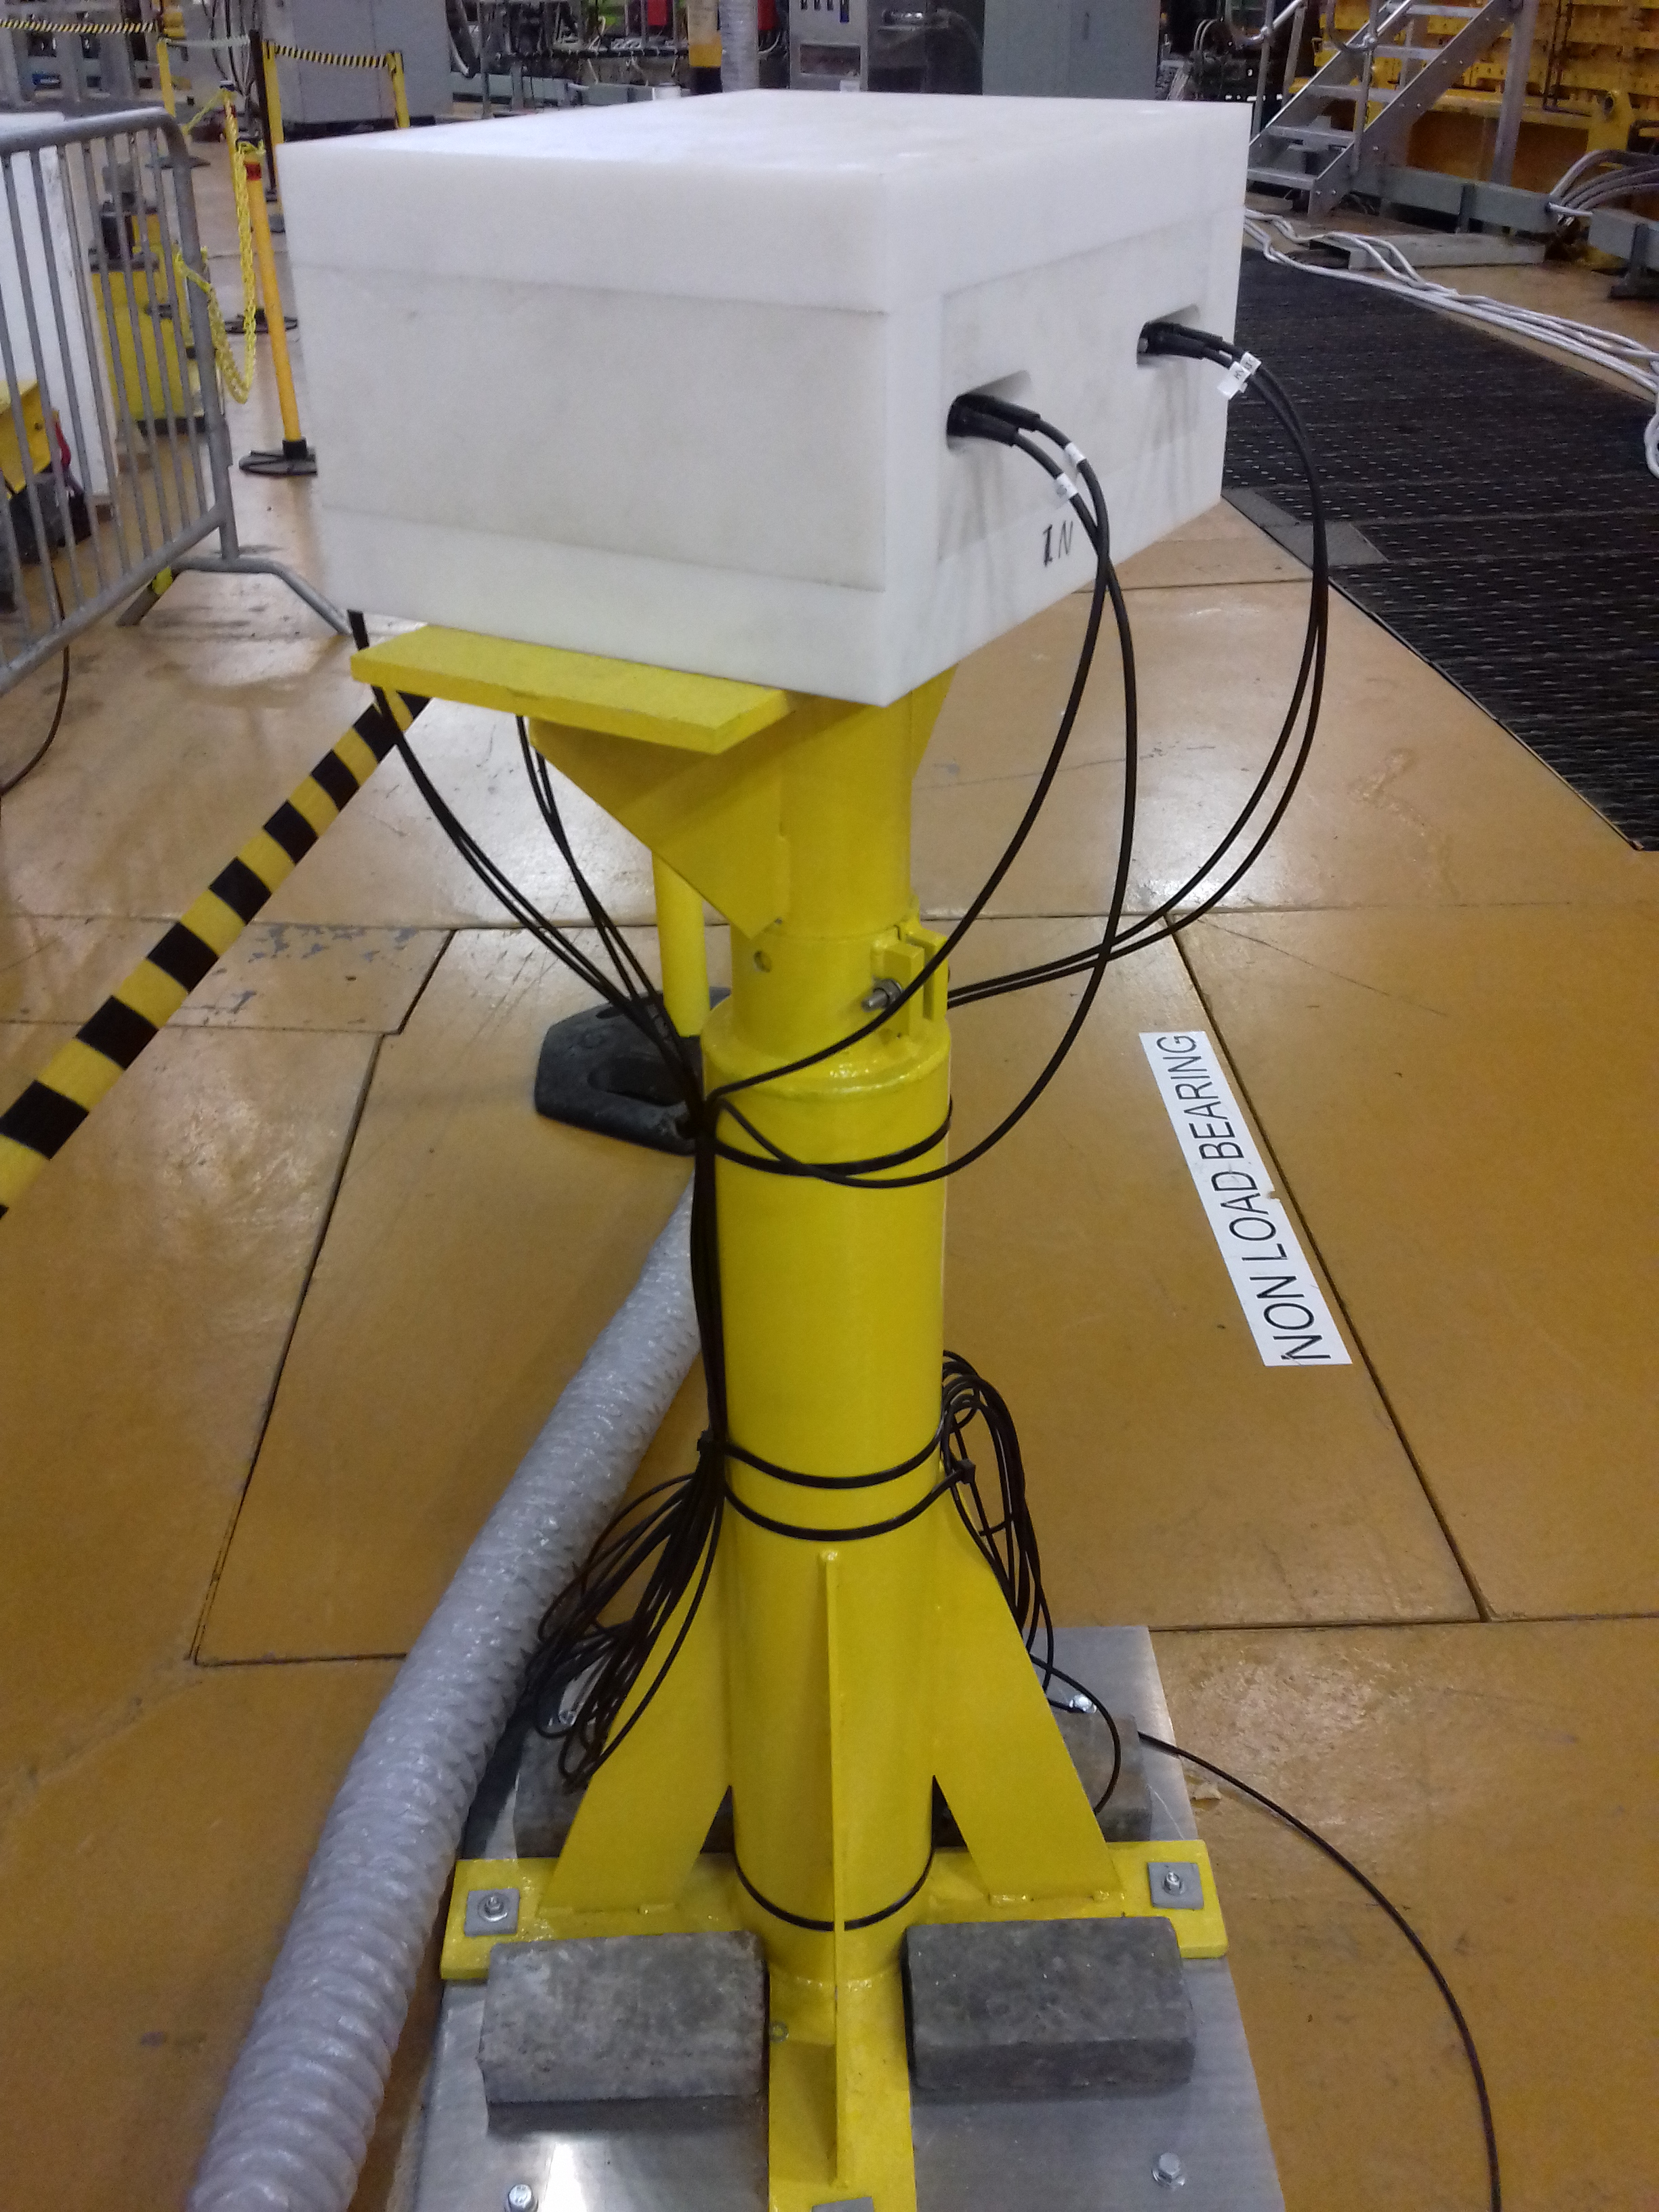
\includegraphics[width=1.0\columnwidth]{./figures/LM4.jpg}
    \caption{The luminosity monitor encapsulated in a 2~inch plastic sarcophagus.}
    \label{fig:LM2}
  \end{center}
\end{figure}


\begin{figure}
  \begin{center}
  \begin{subfigure}
  \centering
    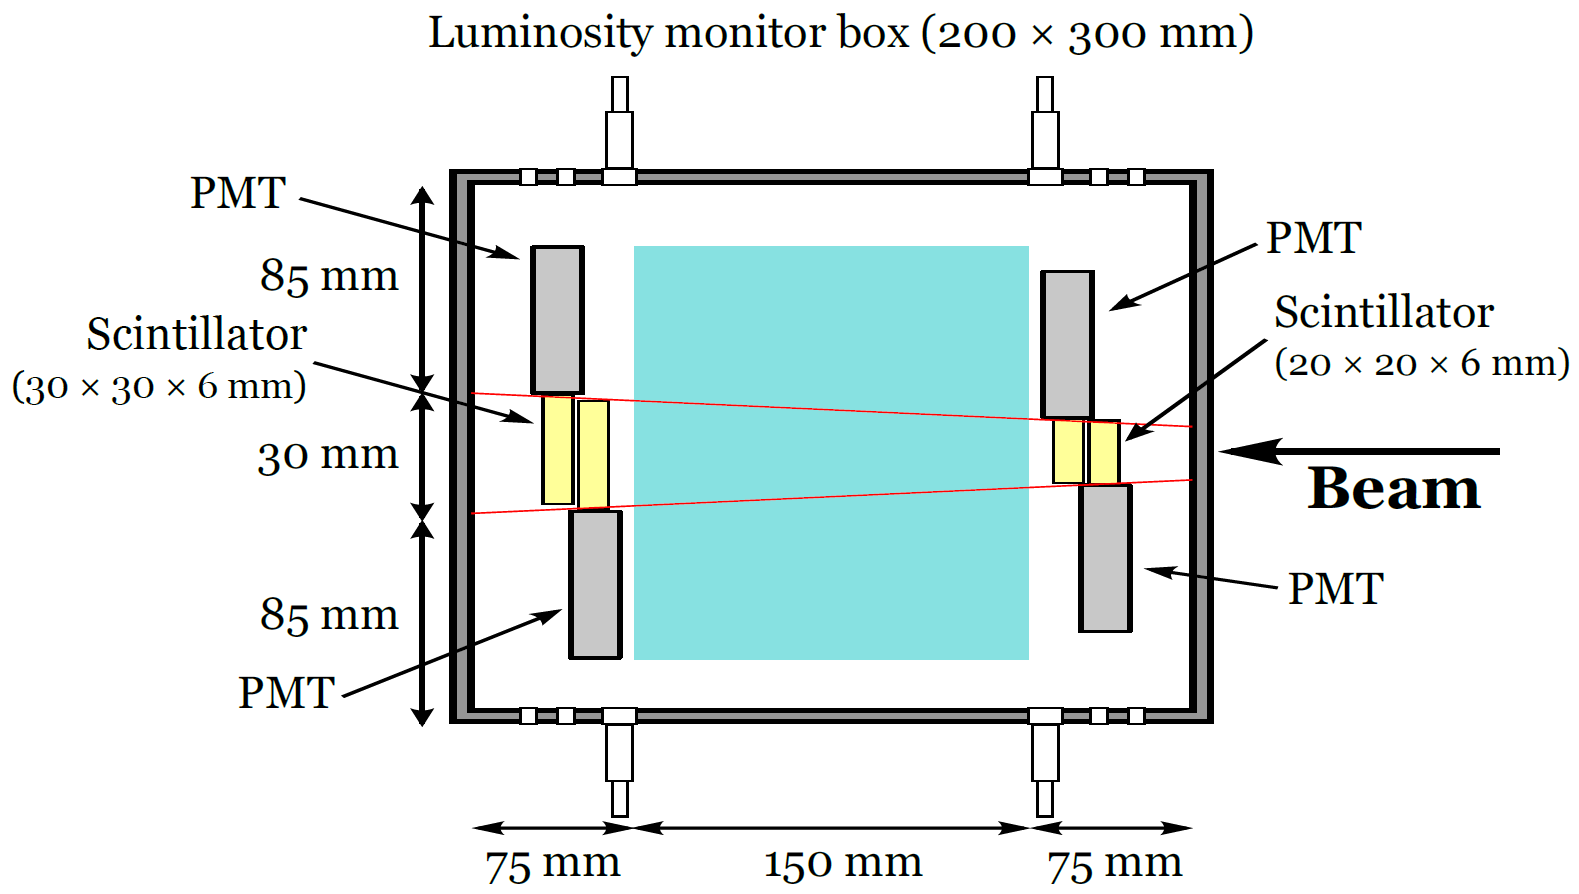
\includegraphics[width=0.59\columnwidth]{./figures/LM2.png}
  \end{subfigure}
  \begin{subfigure}
  \centering
    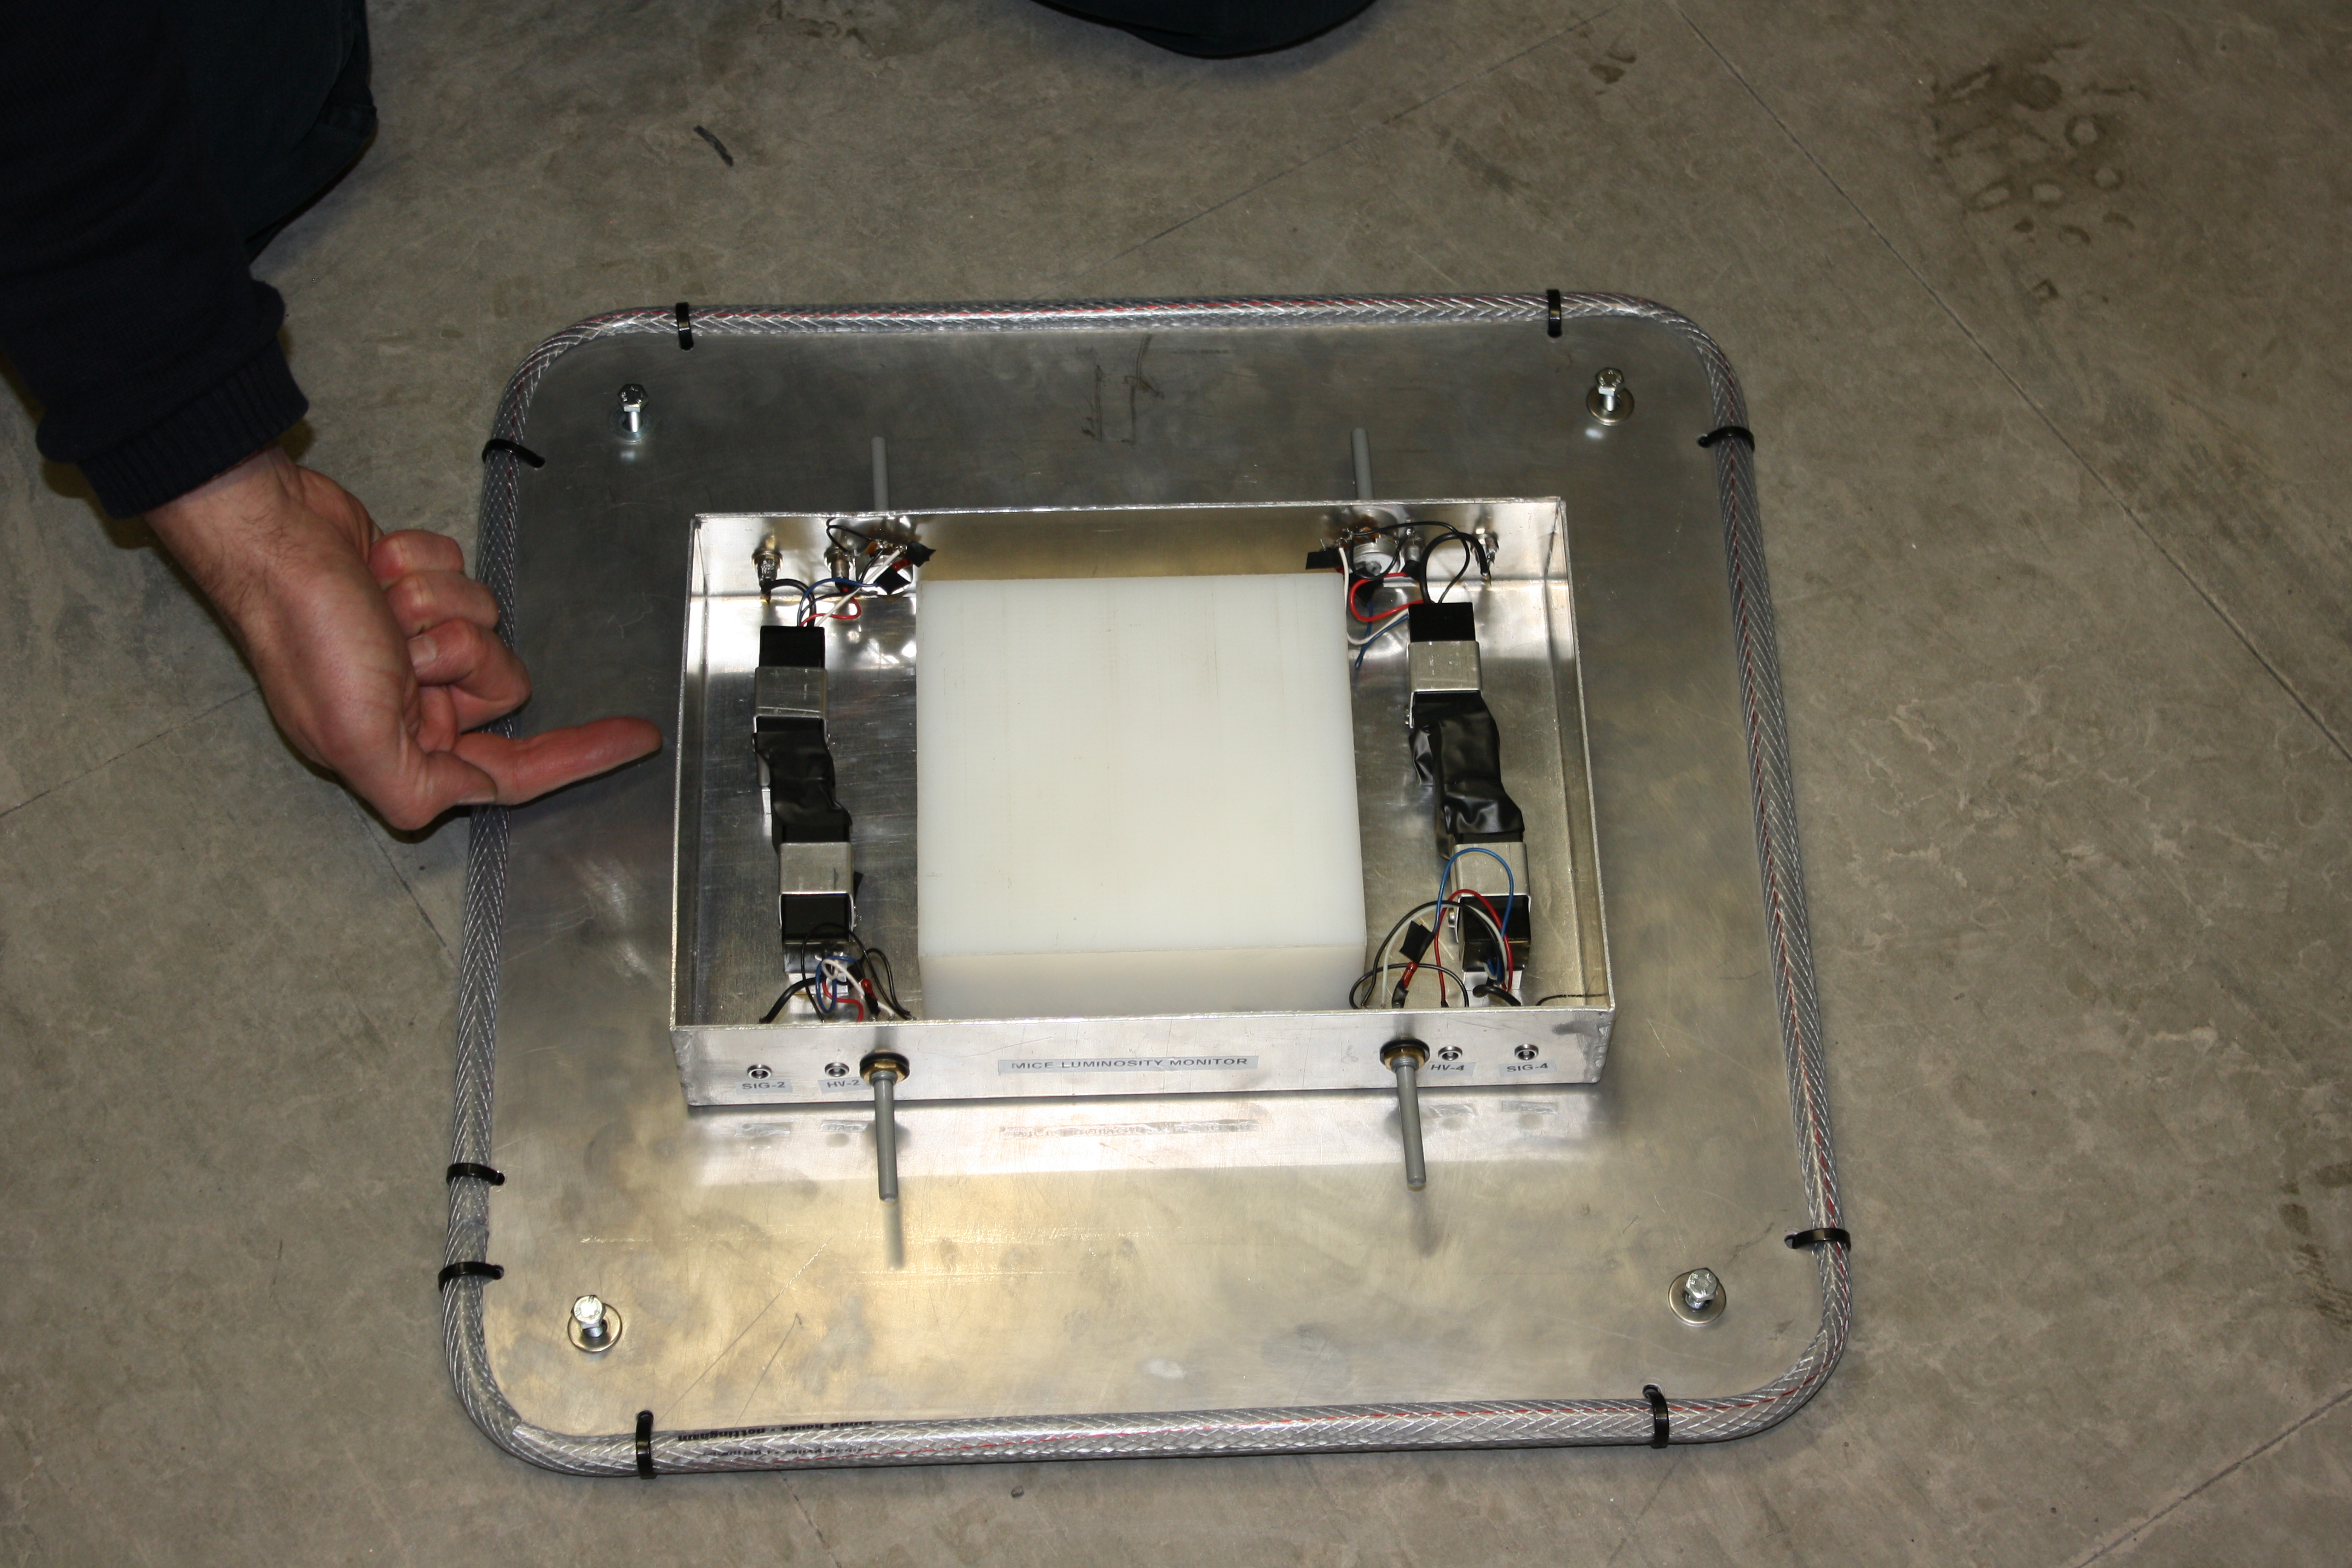
\includegraphics[width=0.39\columnwidth]{./figures/LM3.jpg}
  \end{subfigure}
  \caption{Design of the luminosity monitor (left) and the luminosity monitor box itself (right).}
  \label{fig:LM3}
  \end{center}
\end{figure}

\section{Conclusions}

\begin{thebibliography}{9}
\bibitem{mars} https://mars.fnal.gov/
\bibitem{micenote216} MICE note \#216, http://mice.iit.edu/micenotes/public/pdf/MICE0216/MICE0216.pdf
\bibitem{micenote242} MICE note \#242, http://mice.iit.edu/micenotes/public/pdf/MICE0242/MICE0242.pdf
\bibitem{micenote480} MICE note \#480, http://mice.iit.edu/micenotes/public/pdf/MICE0480/MICE0480.pdf
\bibitem{beampipesurvey1} ISIS Survey Drawing 1-SI-6305-031-01-D, M113 Vacuum Vessel
\bibitem{beampipesurvey2} ISIS Survey Drawing 1-SI-6305-031-02-C, M113 Vacuum Vessel
\bibitem{beampipesurvey3} ISIS Survey Drawing 1-SI-6305-031-03-C, M113 Vacuum Vessel
\bibitem{ISISbeamlinesurvey} ISIS Survey Drawing 0-SI-5100-105-04-I, Essential Geometry of ISIS
\bibitem{MICEsurvey} MICE Beamline Decommissioning Survey Report


\end{thebibliography}

\begin{appendices}
\chapter{ISIS Schematics and Survey Drawings}

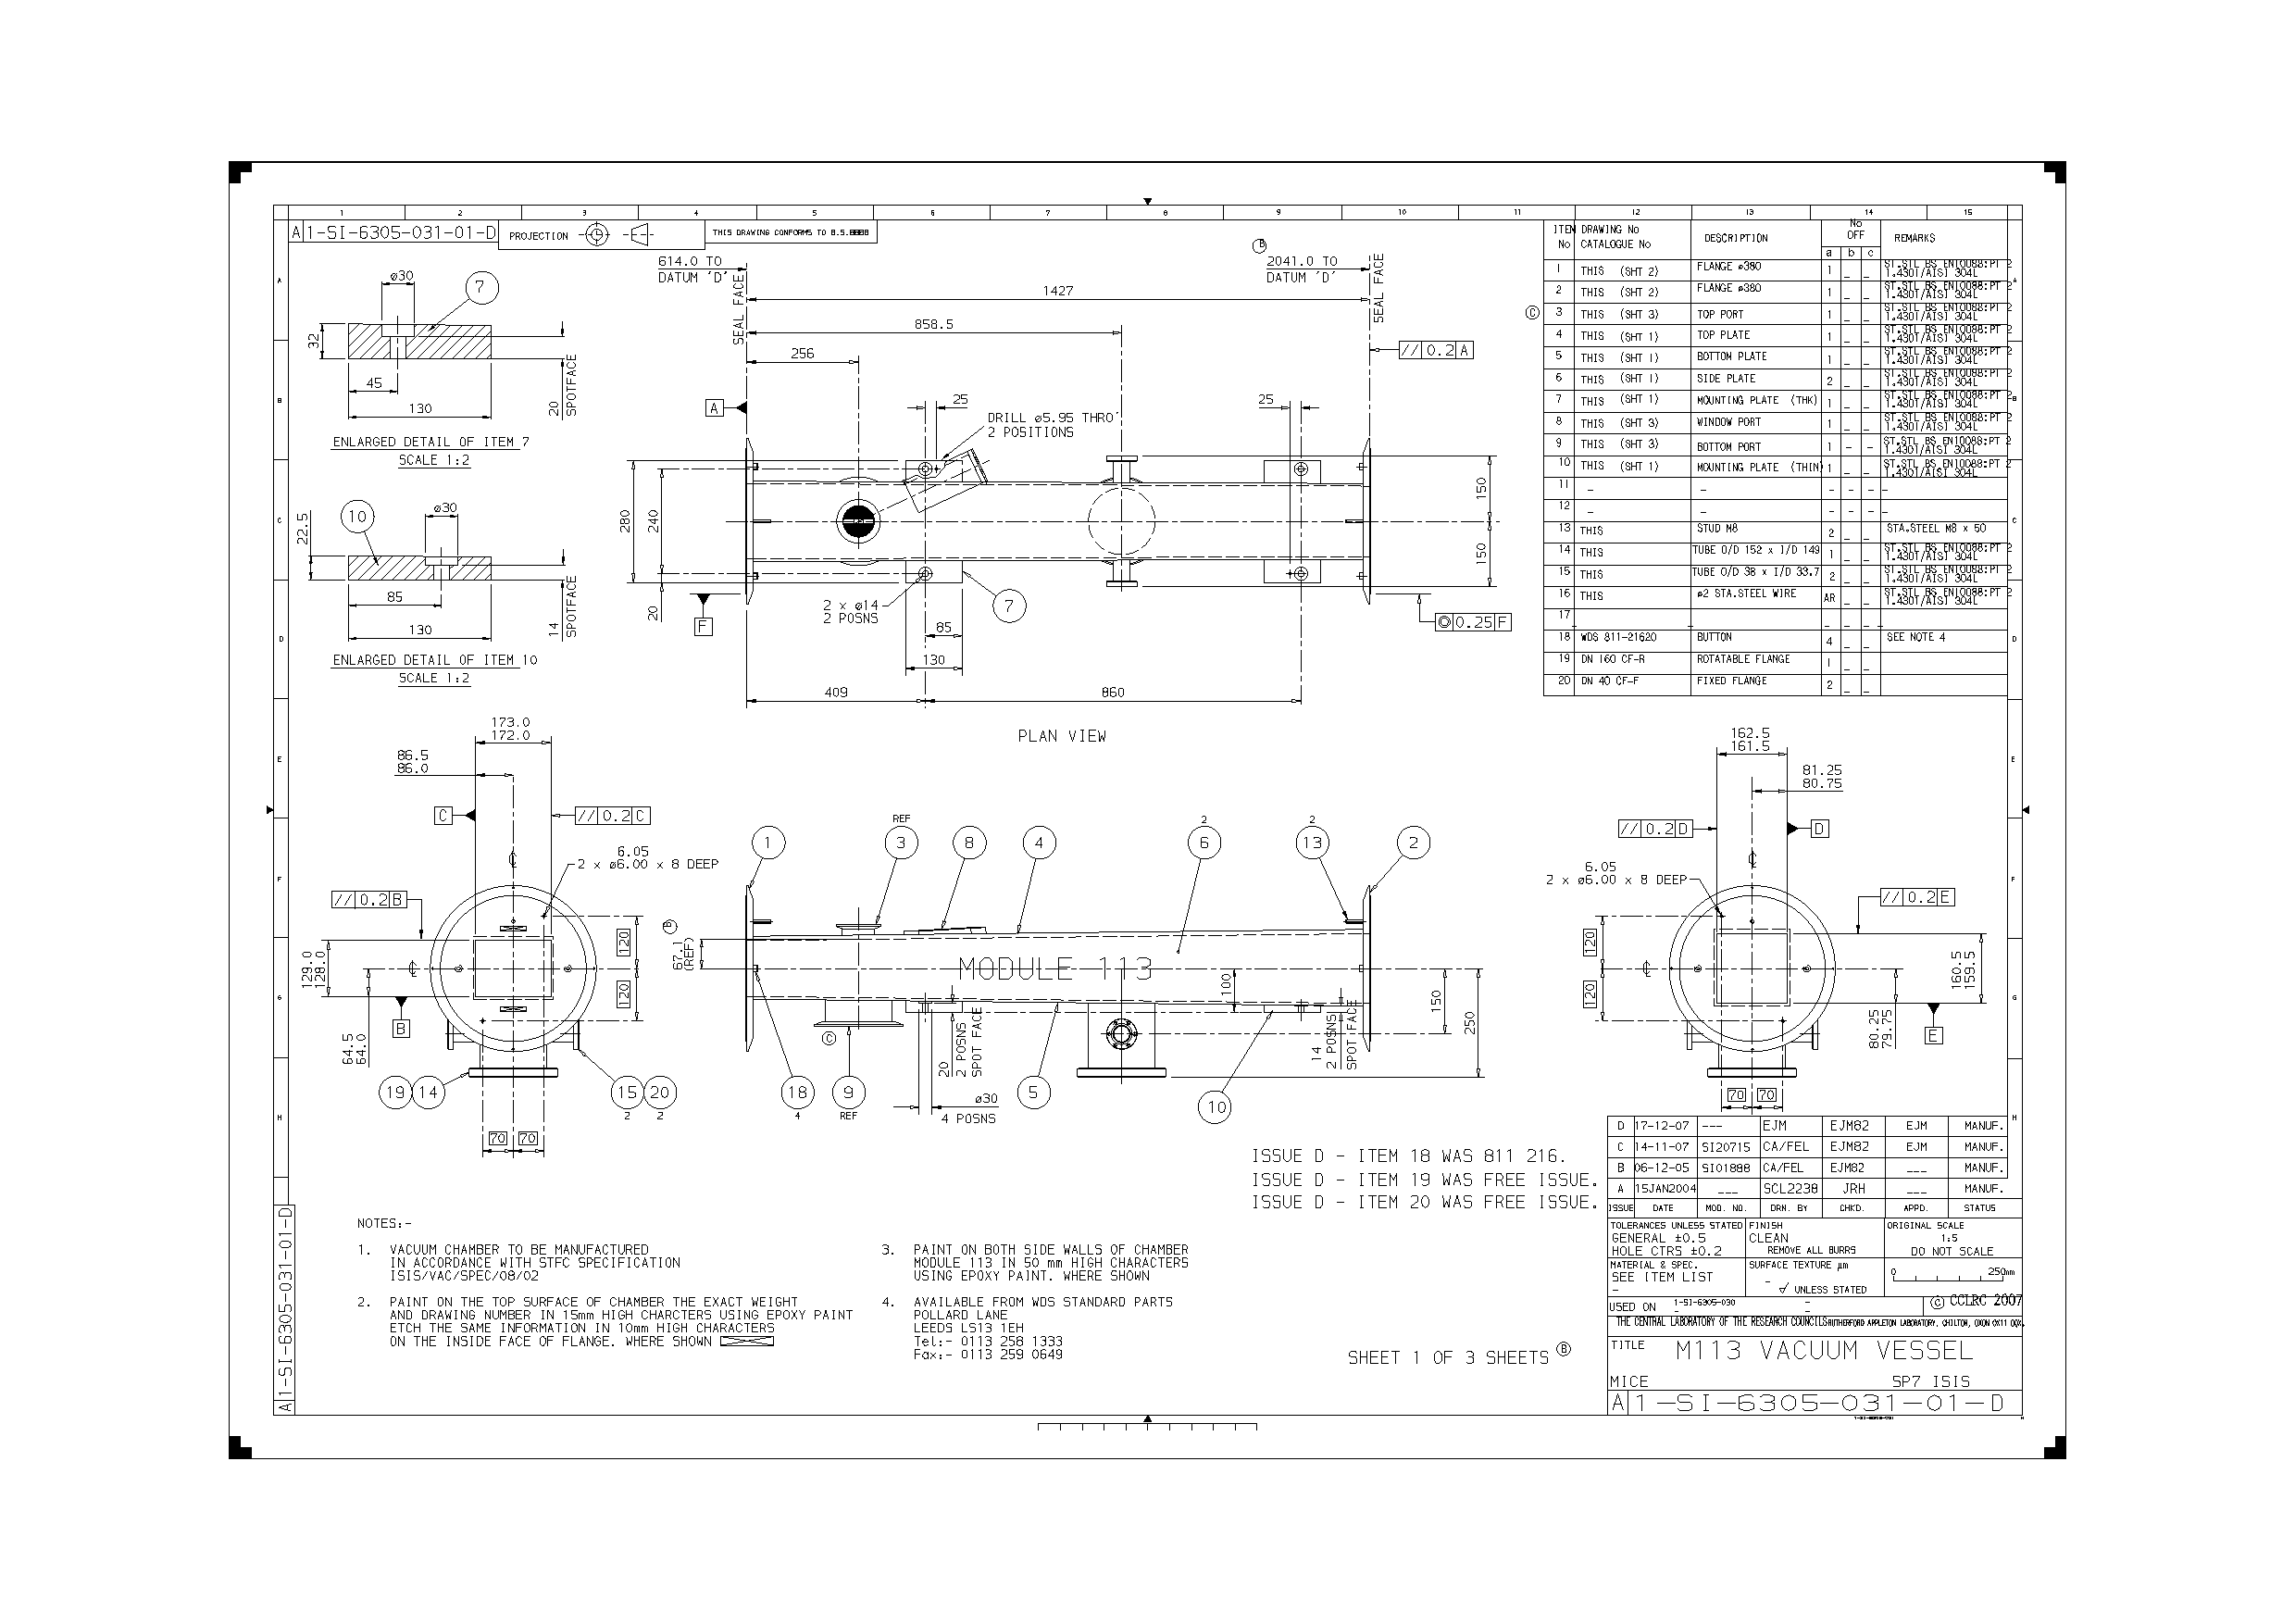
\includepdf{./figures/BeampipeSurvey1.pdf}
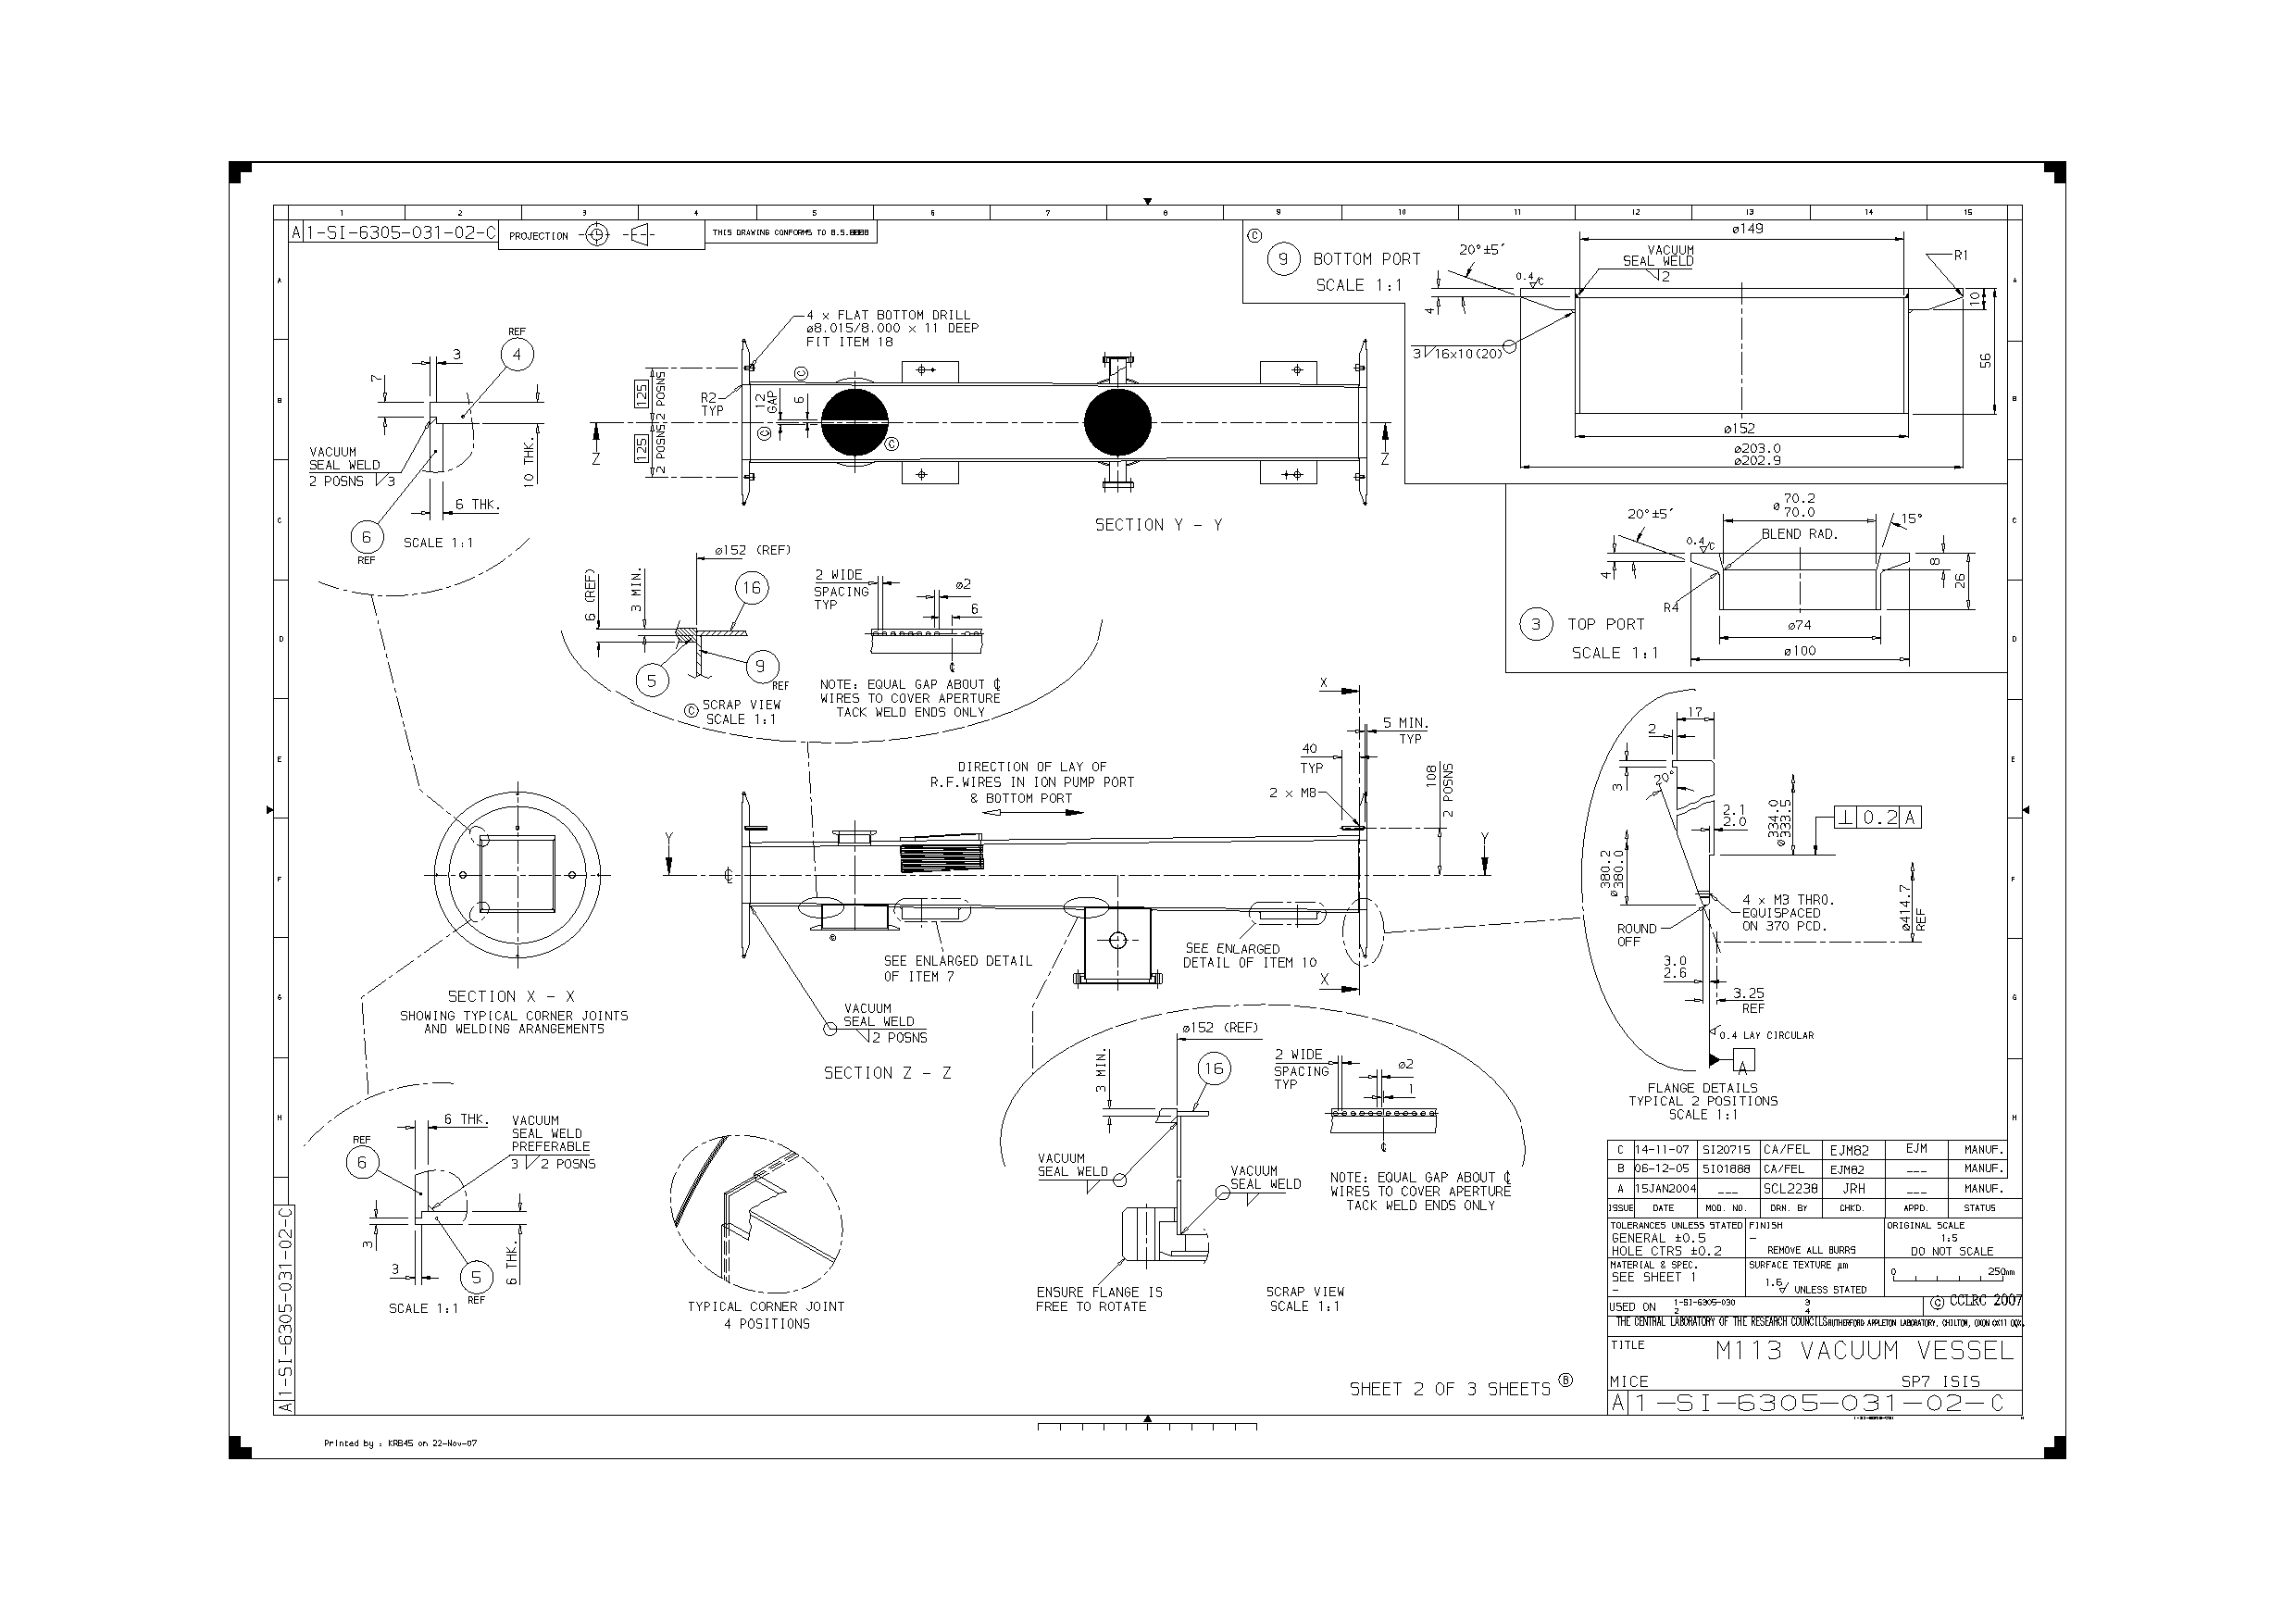
\includepdf{./figures/BeampipeSurvey2.pdf}
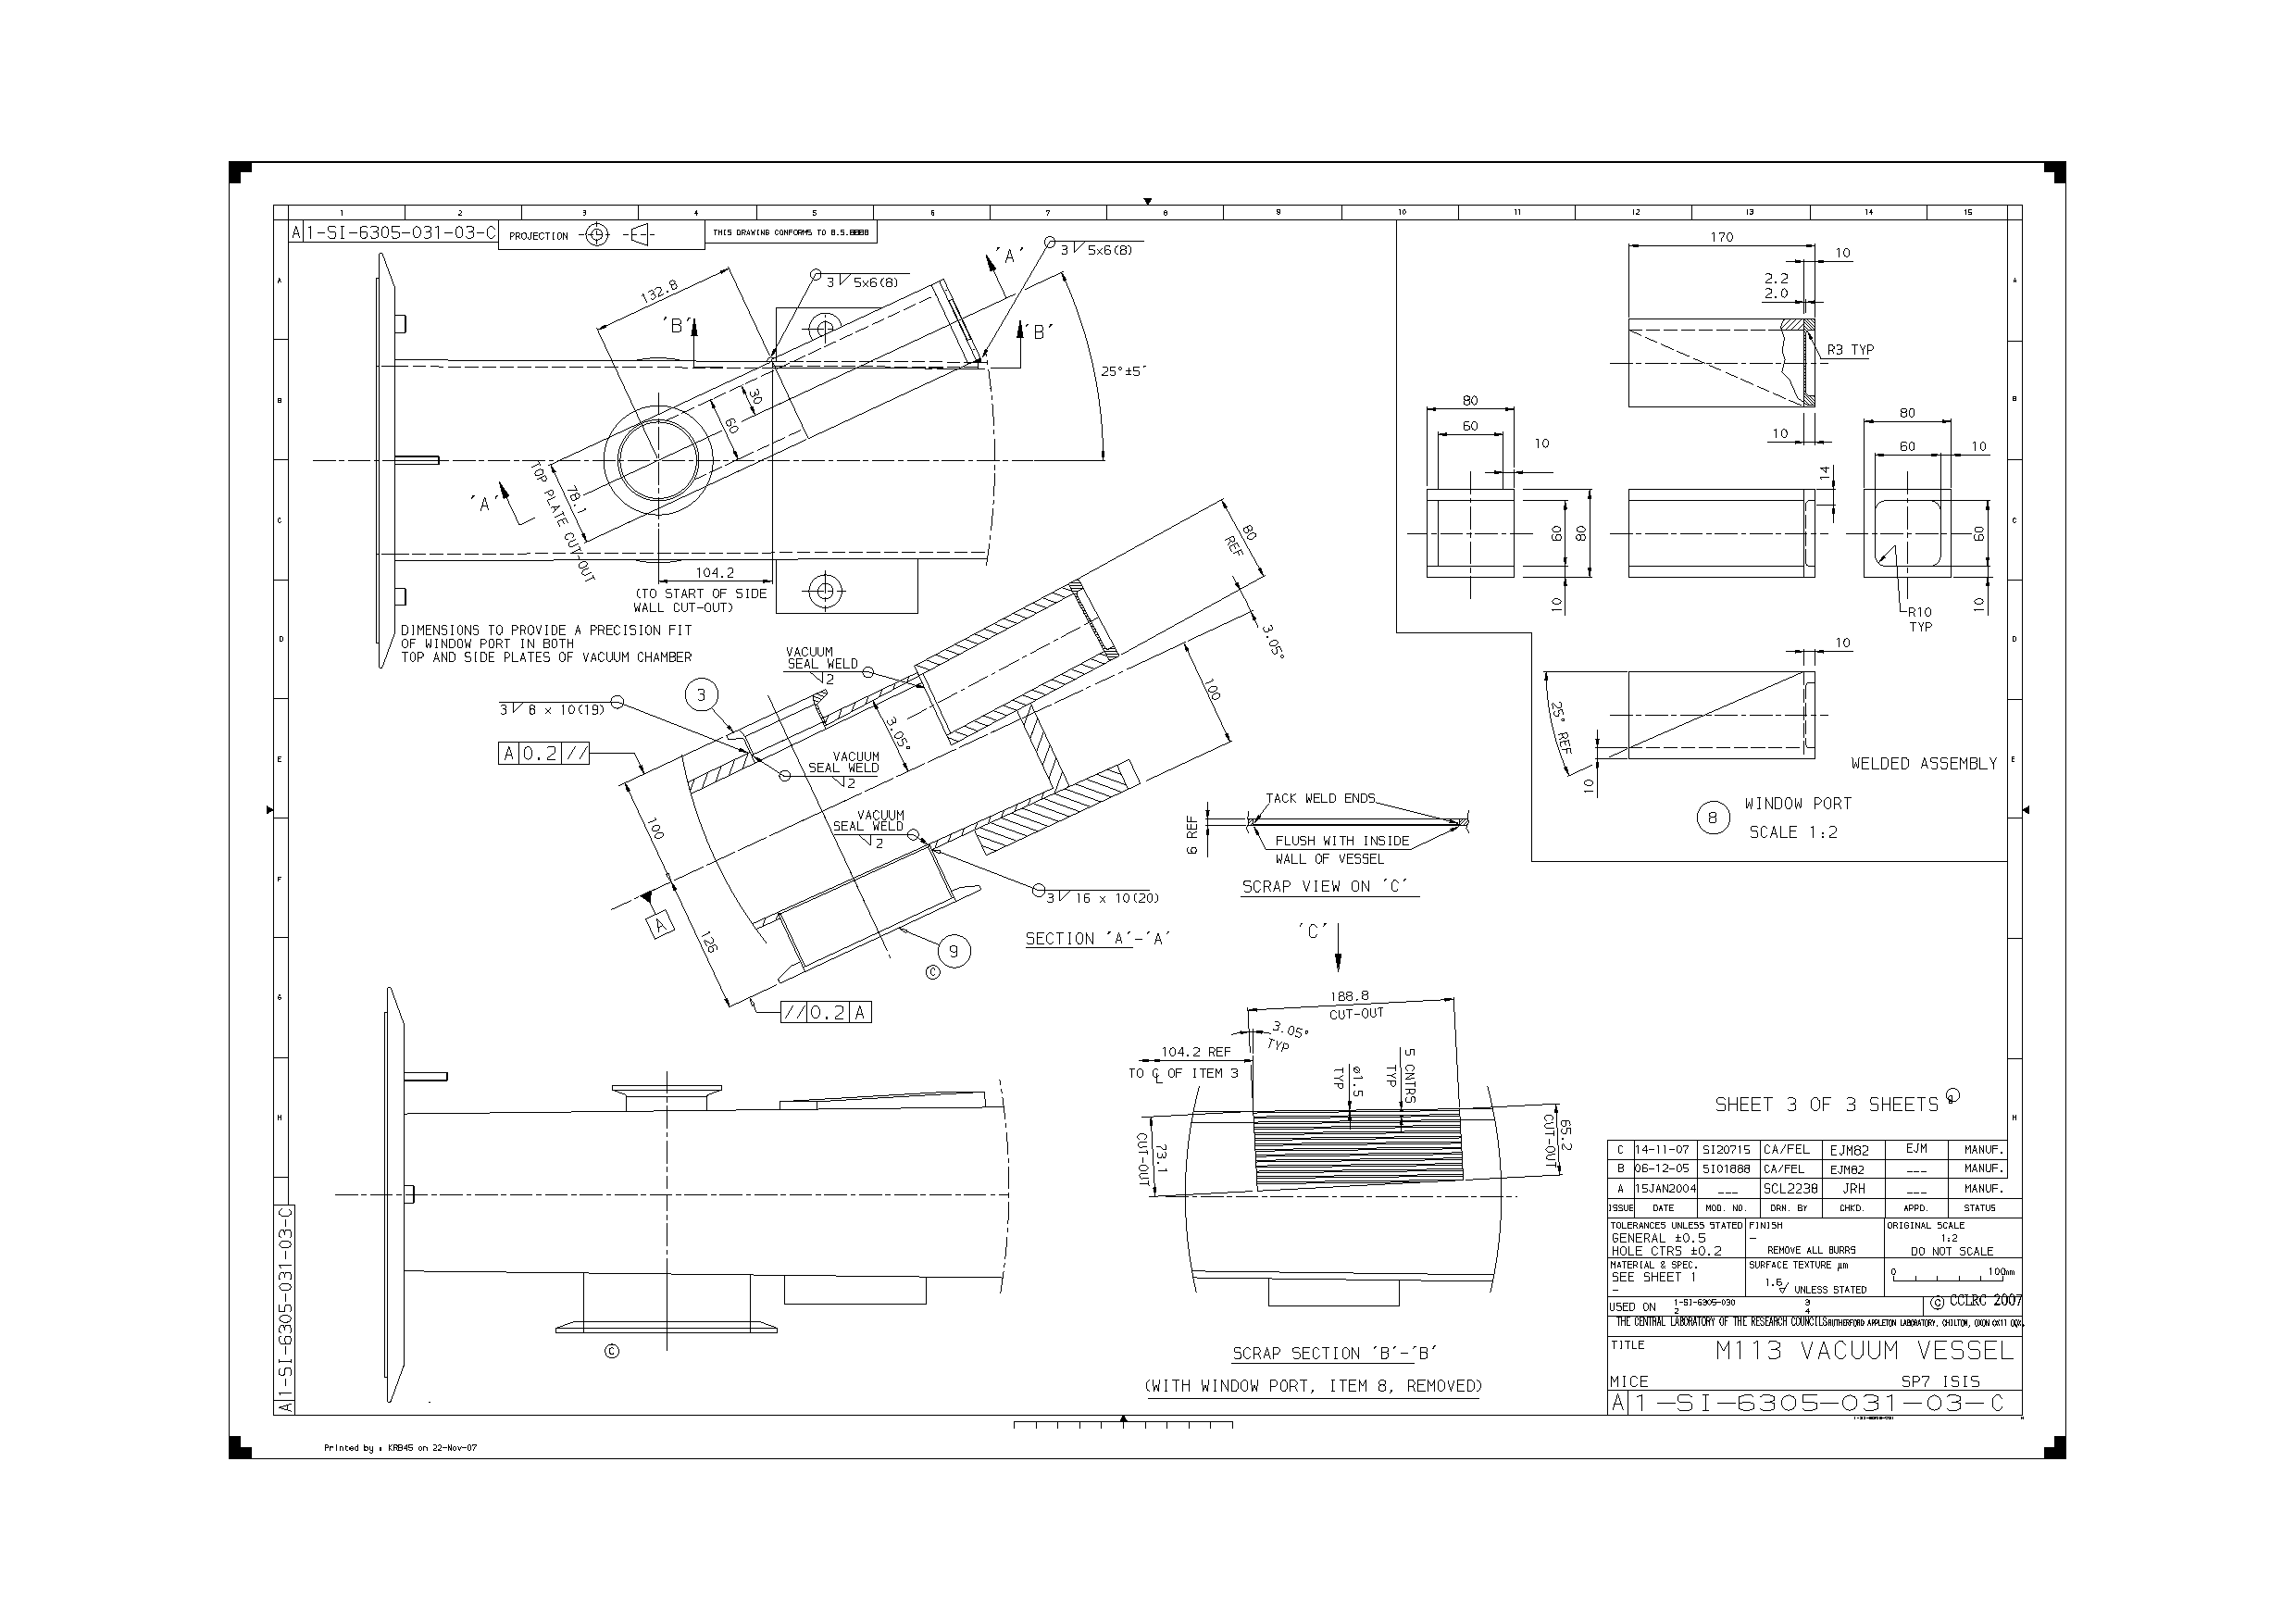
\includepdf{./figures/BeampipeSurvey3.pdf}
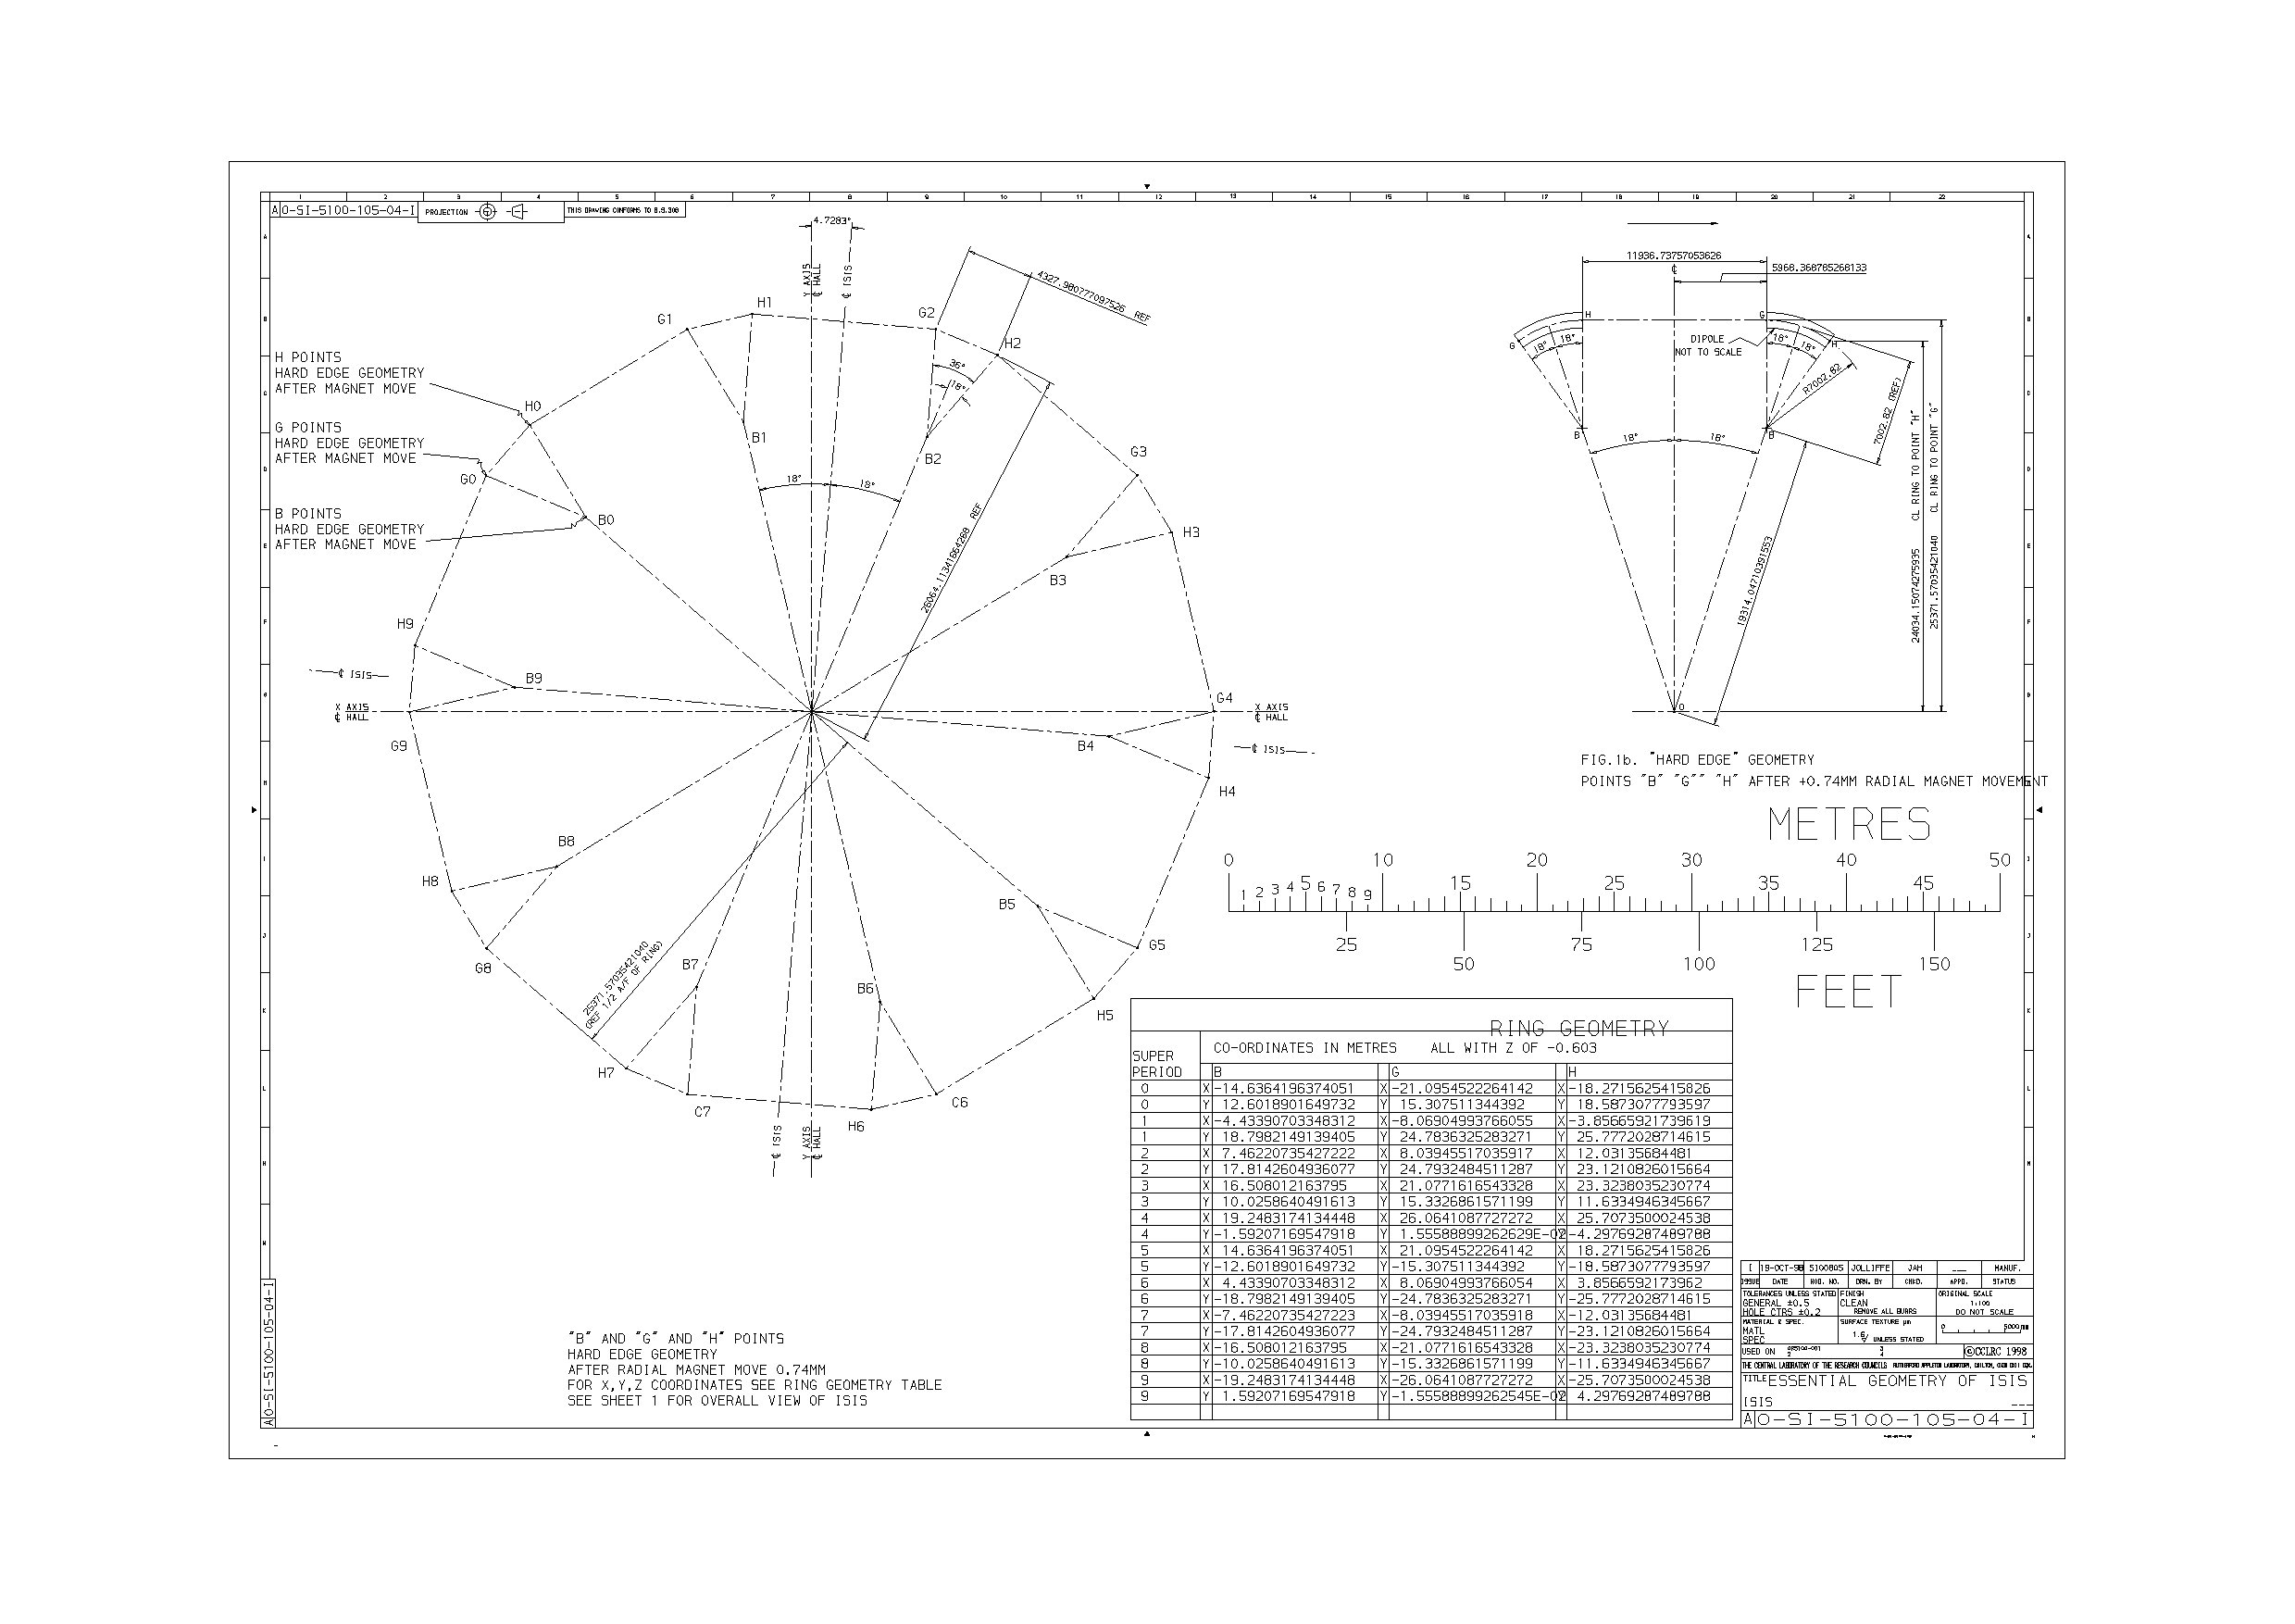
\includepdf{./figures/IsisGeometry.pdf}

\end{appendices}

\end{document}
